\section{Results}
\label{sec:results}

In this section we report the results of the experiments we carried out
to quantify the performance of the reaching movements. Following the proposed strategy, 
in order to reach for the 
target we first need to fixate it, i.e. $\utarget = 0$. Using the available sensor (i.e. vision) the best we can do to precisely reach the target is moving the hand to the fixation point, i.e. $
{\uhand} \longrightarrow 0$. Clearly, the image plane distance $\| \uhand - \utarget \|$ can be used as a rough estimate of the reaching precision, i.e. of the Cartesian distance between the target to be reached and the position of the hand. Specifically, assuming infinite resolution of the camera sensor, if $\| \uhand - \utarget\| = 0$ then the hand has exactly reached the target.

\subsection{Open Loop}
The first attempt to reach the target consists in using the learned forward model 
(\ref{Eq:forward}) and the strategy (\ref{Eq:reaching2})
to choose the arm configuration $\q_{arm}$ which brings the hand to the center 
of the image planes. Clearly, if the forward 
kinematic function (\ref{Eq:forward}) were perfectly represented and if the target were reachable, then we would have 
$\mathbf x_{hand} =  \mathbf x_{target}$, which implies that the target-hand Cartesian distance 
 is zero (see Section \ref{sec:reaching} for details). Therefore, in this ideal case, the open loop 
 strategy already results in $\| \uhand - \utarget \| = 0$. In practice, the model 
 (\ref{Eq:forward}) cannot exactly represent the system's kinematic\footnote{Part of the representational 
 errors are related to the representation of the kinematic function, in this case the
 so called Receptive Field Weighted Regression model. Part are due to the mechanical plays and backlash of the
 mechanical structure.}. Therefore, even tough we can find $\q_{arm}$ such that $\mathbf x_{hand}=
 \hat f_{arm}(\mathbf q_{arm})$ it is not guaranteed that after the movement execution 
 $\| \uhand - \utarget \| = 0$. Figure \ref{Fig:ImagePlaneOpenLoopErrors}
 shows the image plane errors after the execution of the open loop movement. The plot has been obtained
 by fixating a target and performing a series of open loop movements. Each open loop
 movement was different because (\ref{Eq:reaching2}) was solved 
 by choosing a different value $q_{20}$. 


\begin{figure}
  % Requires \usepackage{graphicx}
  \begin{center}
	\begin{tabular}{ccc}
	  \parbox{30mm}{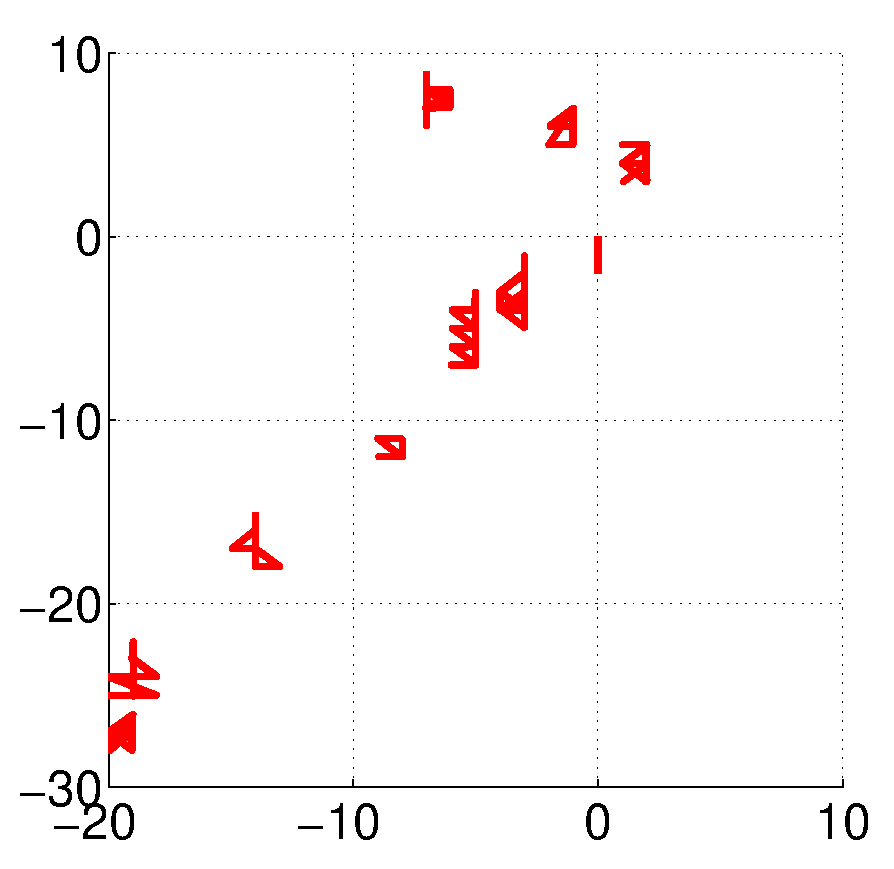
\includegraphics[width=30mm]{Figure/LeftEyeOpenLoop.eps}}  & \hspace{0.1cm} &
	  \parbox{30mm}{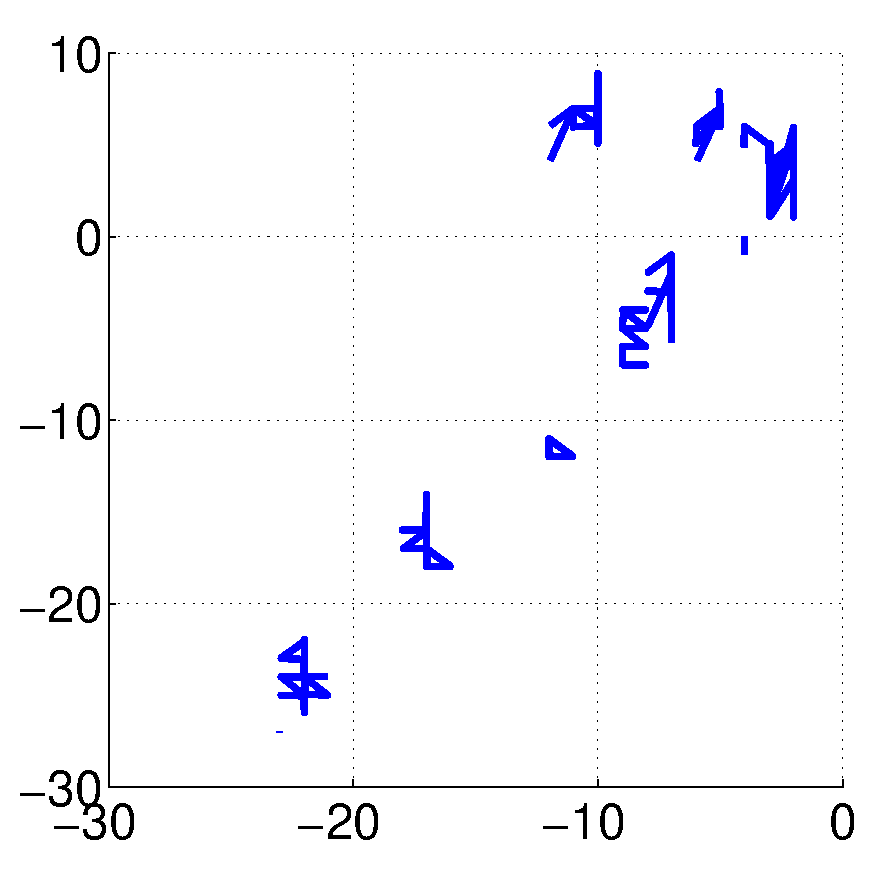
\includegraphics[width=30mm]{Figure/RightEyeOpenLoop.eps}}
	  \\
	  \parbox{30mm}{\centering Left eye } & \hspace{0.1cm} & \parbox{30mm}{\centering Right eye }
	  %	  \end{t\\
	  %	Top view & & Lateral view
  \end{tabular}
\end{center}
\caption{Open loop image plane errors $\uhand$ for different
choices of the redundant variable $q_{20}$. On the horizontal axis 
$u_r$ and $u_l$; vertical axis $v_r$ and $v_l$ (always in pixels).
The hand position in the image plane is represented 
by the small circles.  Each circle corresponds to a different open loop movement, i.e. a different value of $q_{20}$.
}\label{Fig:ImagePlaneOpenLoopErrors}
 \end{figure}

\subsection{Closed Loop}

The residual image plane errors 
due to imperfections in the forward kinematic model can be reduced by a visual closed loop
control strategy (\ref{Eq:ClosedLoopStrategy}), started immediately after the open loop phase. Relatively weak conditions on the learned 
Jacobian \cite{Samson91robot} guarantee the convergence of the image plane errors $\uhand$ to zero, and therefore
the convergence of the hand $\xhand$ on the target $\xtarget$. Figures
\ref{Fig:ImagePlaneClosedLoopErrors}, %\ref{Fig:TimeResponseClosedLoopErrors}, 
\ref{Fig:TimeResponseOpenClosedLoopErrors} and \ref{Fig:TimeResponseOpenClosedLoop}  
show how the hand is actually driven to the 
exact image center in both the image planes. The closed loop controller 
improves the accuracy of the reaching movement, but at the cost of a slower 
execution speed (see Figure \ref{Fig:TimeResponseOpenClosedLoop}); faster
executions couldn't be obtained by increasing the control loop gains, due to
the frame rate (thirty milliseconds) and the delays in the visual processing (hand localization and tracking).
Finally, it is important to notice 
the quasi-linearity of the path followed by the hand 
(see Figure \ref{Fig:ImagePlaneClosedLoopErrors}). This linearity denotes 
a good accuracy of the learned Jacobian.

\begin{figure}[th!]
  % Requires \usepackage{graphicx}
  \begin{center}
	\begin{tabular}{ccc}
	  \parbox{30mm}{\includegraphics[width=30mm]{Figure/LeftEyeClosedLoop.eps}}  & \hspace{.1cm} &
	  \parbox{30mm}{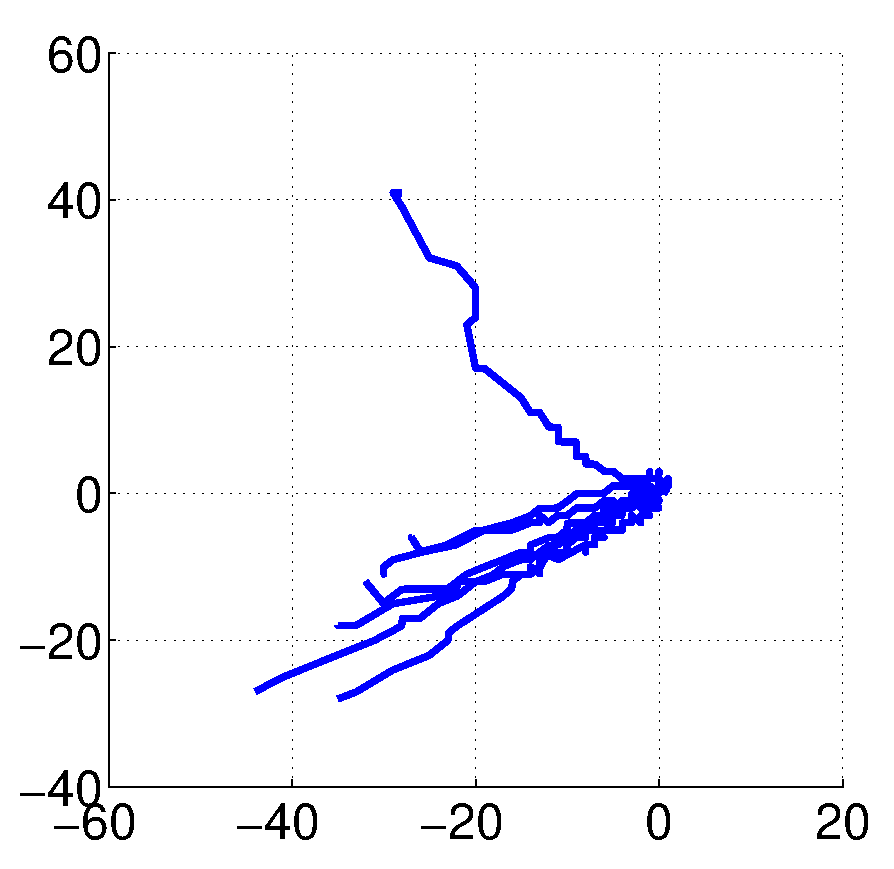
\includegraphics[width=30mm]{Figure/RightEyeClosedLoop.eps}}
	  \\
	  \parbox{30mm}{\centering Left eye } & \hspace{0.1cm} & \parbox{30mm}{\centering Right eye }
	  %	  \end{t\\
	  %	Top view & & Lateral view
  \end{tabular}
\end{center}
\caption{Traces of different closed loop control actions. Each trace correspond to a different Cartesian position of the target to be reached (which 
is always at the center of the image planes). All the traces end up in the image center thus indicating that the visual errors are completely eliminated by the closed loop controller.}\label{Fig:ImagePlaneClosedLoopErrors}
  \end{figure}

%\begin{figure}
%  % Requires \usepackage{graphicx}
%  \begin{center}
%	\begin{tabular}{ccc}
%	  \parbox{30mm}{\includegraphics[width=30mm]{Figure/TimeReponseLeftClosedLoop.eps}}  & \hspace{.1cm} &
%	  \parbox{30mm}{\includegraphics[width=30mm]{Figure/TimeReponseRightClosedLoop.eps}}
%	  \\
%	  \parbox{30mm}{\centering Left eye } & \hspace{0.1cm} & \parbox{30mm}{\centering Right eye }
%	  %	  \end{t\\
%	  %	Top view & & Lateral view
%  \end{tabular}
%\end{center}
%\caption{Time response of the closed loop controller. Solid lines: hand horizontal position in the left ($u_l$) and right ($u_r$). Dashed lines: vertical position, $v_l$ and $v_r$.}\label{Fig:TimeResponseClosedLoopErrors}
%  \end{figure}


\begin{figure}[th!]
  % Requires \usepackage{graphicx}
  \begin{center}
	\begin{tabular}{ccc}
	  \parbox{30mm}{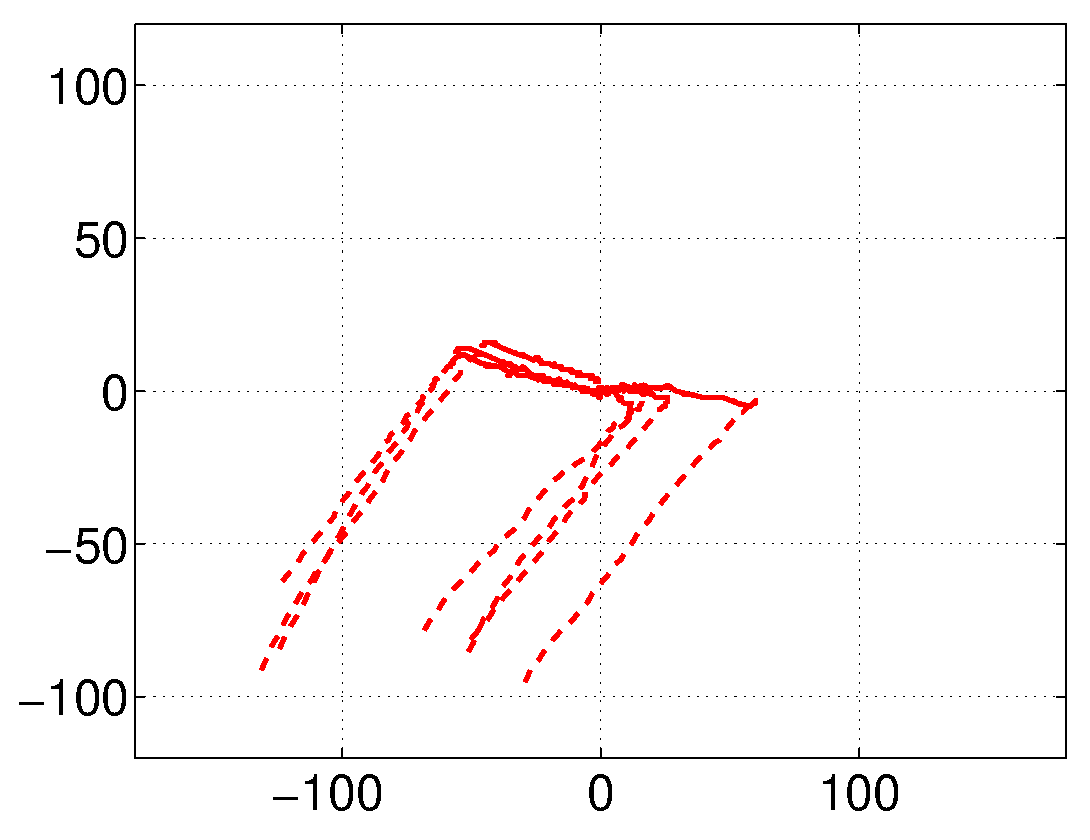
\includegraphics[width=30mm]{Figure/LeftEyeOpenClosedLoop.eps}}  & \hspace{.1cm} &
	  \parbox{30mm}{\includegraphics[width=30mm]{Figure/RightEyeOpenClosedLoop.eps}}
	  \\
	  \parbox{30mm}{\centering Left eye } & \hspace{.1cm} & \parbox{30mm}{\centering Right eye }
	  %	  \end{t\\
	  %	Top view & & Lateral view
  \end{tabular}
\end{center}
\caption{Movement of the hand on the image planes (320$\times$240)
during the execution of different reaching actions. 
Solid line: closed loop. Dashed trace: open loop. Clearly the open loop movement drives the hand to the target (the image centers) with a 
relatively small error. The closed loop phase reduces this error to zero.}\label{Fig:TimeResponseOpenClosedLoopErrors}
  \end{figure}
  
  \begin{figure}[th!]
  % Requires \usepackage{graphicx}
  \begin{center}
	\begin{tabular}{ccc}
	  \parbox{30mm}{\includegraphics[width=30mm]{Figure/LeftEyeOpenClosedLoopTimeResponse.eps}}  & \hspace{.1cm} &
	  \parbox{30mm}{\includegraphics[width=30mm]{Figure/RightEyeOpenClosedLoopTimeResponse.eps}}
	  \\
	  \parbox{30mm}{\centering Left eye } & \hspace{.1cm} & \parbox{50mm}{\centering Right eye }
	  %	  \end{t\\
	  %	Top view & & Lateral view
  \end{tabular}
\end{center}
\caption{Time response of the closed loop and open loop strategy. Solid lines: $u_r$ and $u_l$. Dashed lines: $v_r$ and $v_l$. Remarkably, the open loop phase is faster but does not drive the hand exactly on the target. The closed loop is slower but more accurate.}\label{Fig:TimeResponseOpenClosedLoop}
\end{figure}


\subsection{Superimposed Open and Closed Loop}

Finally, we tested an alternative control strategy based on activating the closed loop 
phase immediately after the hand becomes visible on both image planes. This second strategy
is such that the open a closed loop strategies will be active at the same time for a 
certain amount of time. 
\newpage 
The structure is based on a classical control scheme, which can be represented as follows:

\begin{figure}[th!]
\begin{center}
\includegraphics[scale = 0.25]{Figure/OpenVSClosedLoop.eps}
\end{center}
\end{figure}

Practically, the feedforward control corresponds to the open loop part of the reaching movement.
It is activated exactly as described in Section \ref{sec:openReaching} and therefore it does not
require the hand to be visible in the image plane. The feedback control
instead corresponds to the closed loop part of the movement and can be activated when the hand
has been localized in both the image planes. Practically, the final solution can be described by the 
following scheme:

\begin{figure}[th!]
\begin{center}
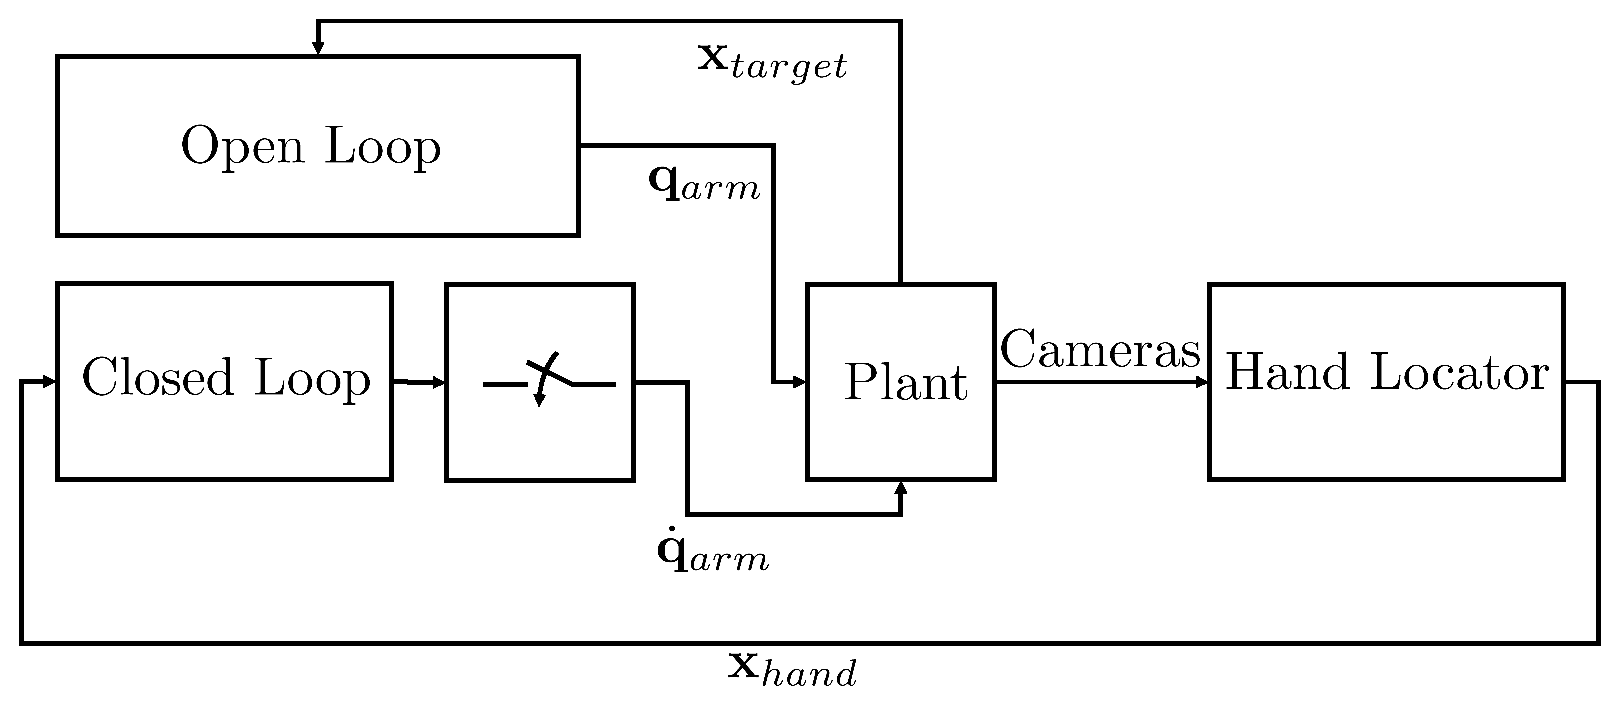
\includegraphics[scale = 0.25]{Figure/OpenVSClosedLoopSwitch.eps}
\end{center}
\end{figure}

Clearly, when both the open and closed loop controllers are active, the system receives position 
and velocity control simultaneously\footnote{A position command ${\mathbf q}_{arm,d}$ is 
always translated into a trajectory following command by moving 
the hand along a trajectory $\mathbf q_{arm}(t)$, $t \in [0, T]$ such that: $T$ is the execution time,
$\mathbf q_{arm}(0)$ is the arm position when the command is received, $\mathbf q_{arm}(T) = {\mathbf q}_{arm,d}$
is the desired final position, $\dot {\mathbf q}_{arm}(t) = 0$, $ \forall t > T$. If a velocity command $\dot {\mathbf q}_{arm,d}$ is received while executing a position
command $\mathbf q_{arm}(t)$, the original velocity command is transformed into a new one, nominally
$\dot {\mathbf q}_{arm} = \dot {\mathbf q}_{arm}(t) + \dot {\mathbf q}_{arm, d}$.}. 

A comparison between this control strategy and the one proposed in Section \ref{Eq:ClosedLoop}
is given in Figure \ref{Fig:TimeResponseOpenVSClosedLoopErrors} and \ref{Fig:TimeResponseOpenVSClosedLoop}. 
The second control strategy clearly outperforms the first one. As a matter of fact, the image plane movement (Figure \ref{Fig:TimeResponseOpenVSClosedLoopErrors})
is much more regular resulting in a unique linear movement instead of begin divided into two segments. Secondly, the
execution time is clearly reduced as it can be noted in Figure \ref{Fig:TimeResponseOpenVSClosedLoop}.


\begin{figure}
  % Requires \usepackage{graphicx}
  \begin{center}
	\begin{tabular}{ccc}
	  \parbox{30mm}{\includegraphics[width=30mm]{Figure/LeftEyeOpenVSClosedLoop.eps}}  & \hspace{.1cm} &
	  \parbox{30mm}{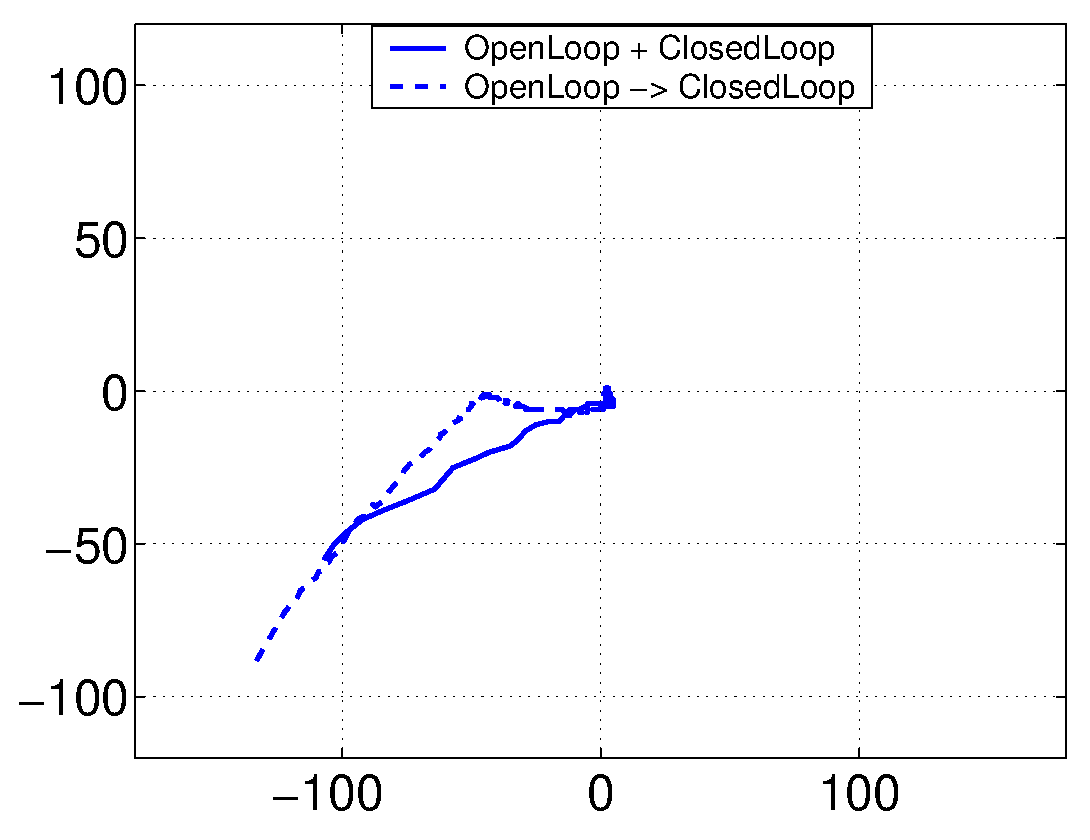
\includegraphics[width=30mm]{Figure/RightEyeOpenVSClosedLoop.eps}}
	  \\
	  \parbox{30mm}{\centering Left eye } & \hspace{.1cm} & \parbox{30mm}{\centering Right eye }
	  %	  \end{t\\
	  %	Top view & & Lateral view
  \end{tabular}
\end{center}
\caption{Movement of the hand on the image planes ($320 \times 240$)
during the execution of a single reaching movement. Dashed line: hand movement
during an open loop movement followed by a closed loop phase. Solid line: hand movement during 
the superposition of open and closed loop strategies.}\label{Fig:TimeResponseOpenVSClosedLoopErrors}
  \end{figure}
  
  \begin{figure}
  % Requires \usepackage{graphicx}
  \begin{center}
	  \parbox{40mm}{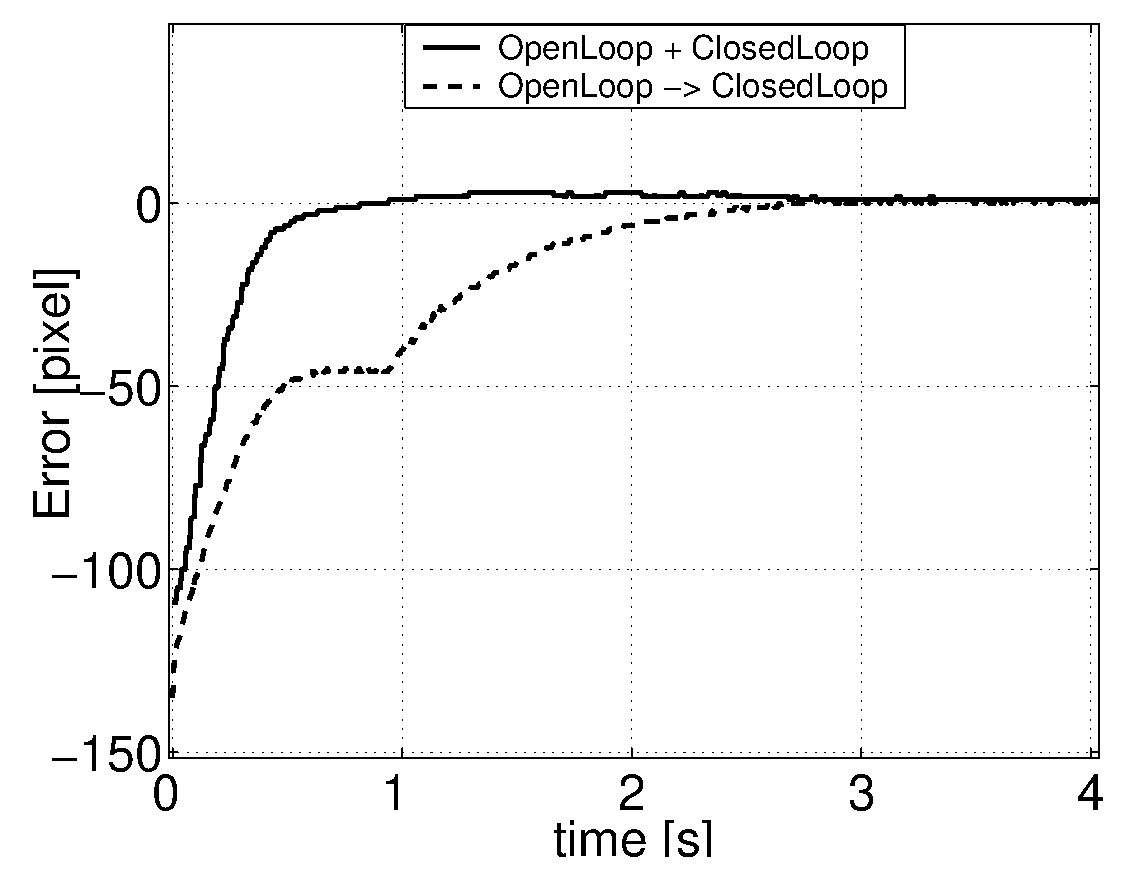
\includegraphics[width=40mm]{Figure/OpenVSClosedLoopTimeResponse1.eps}}
  \end{center}
\caption{Time response of the image plane position $u_l$. Dashed line: hand movement
during an open loop movement followed by a closed loop phase. Solid line: superposition of open and closed loop strategies.
 Remarkably, this second control architecture results in a faster response because when the hand becomes visible it is 
directly driven to the target without waiting for the open loop phase end.}\label{Fig:TimeResponseOpenVSClosedLoop}
  \end{figure}

\subsection{Null space movement}

In order to validate the quality of the Jacobian estimation, we tested the effects of a null space movement 
on the primary task (keeping $\uhand = 0$) as proposed in \cite{Mansard06jacobian}. A simple way to perform this testing is the following control strategy:
\begin{equation} \label{Eq:ClosedLoopStrategyRedundant}
\mathbf{\dot q}_{arm}=-k_1 \cdot \jacobian^\# \uhand + k_2 (I - \jacobian^\# \jacobian) \mathbf w, 
\end{equation}
where $I \in \mathbb R^{4 \times 4}$ is the identity matrix, $\mathbf w \neq 0$ is a 
randomly chosen vector in $\mathbb R^4$ and $k_1$, $k_2$ are positive constants. 
Ideally, the strategy (\ref{Eq:ClosedLoopStrategyRedundant}) should allow arm movements 
$\mathbf{q}_{arm} \neq 0$ while leaving the hand position $\uhand$ unperturbed. Practically we observed 
a minimal image plane movement (Figure \ref{Fig:RedundancyImagePlane})
as oppposed to a relatively large arm movement (Figure \ref{Fig:RedundancyArm}). These results 
further prove the quality of our Jacobian estimation.

\begin{figure}
  % Requires \usepackage{graphicx}
  \begin{center}
	\begin{tabular}{ccc}
	  \parbox{30mm}{\includegraphics[width=30mm]{Figure/RedundancyLeft.eps}}  & \hspace{.1cm} &
	  \parbox{30mm}{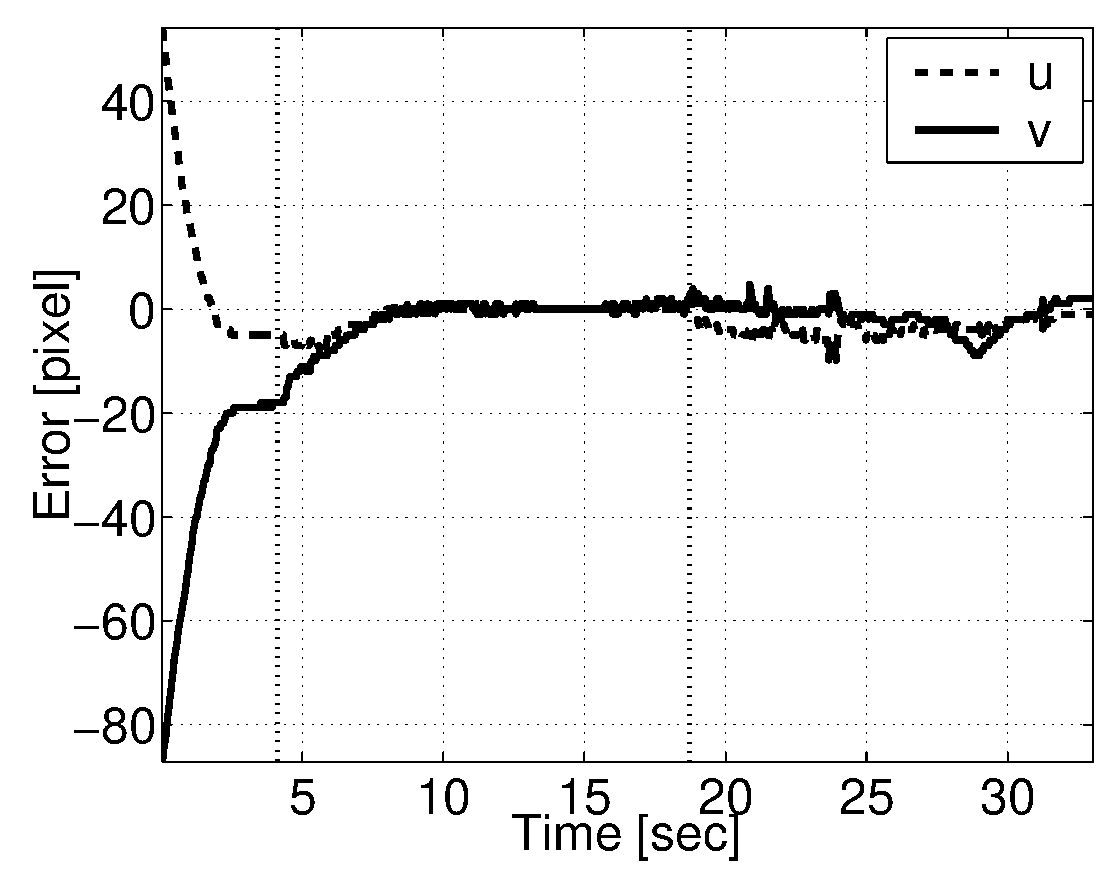
\includegraphics[width=30mm]{Figure/RedundancyRight.eps}}
	  \\
	  \parbox{30mm}{\centering Left eye } & \hspace{.1cm} & \parbox{30mm}{\centering Right eye }
	  %	  \end{t\\
	  %	Top view & & Lateral view
  \end{tabular}
\end{center}
\caption{Image plane movements during a three phase reaching. 
First the open loop, then the closed loop and finally a movement 
in the null space of the given task (keeping the hand in fixations). 
Each phase is delimited by a vertical dotted line.
}\label{Fig:RedundancyImagePlane}
  \end{figure}
  
  \begin{figure}
  % Requires \usepackage{graphicx}
  \begin{center}
	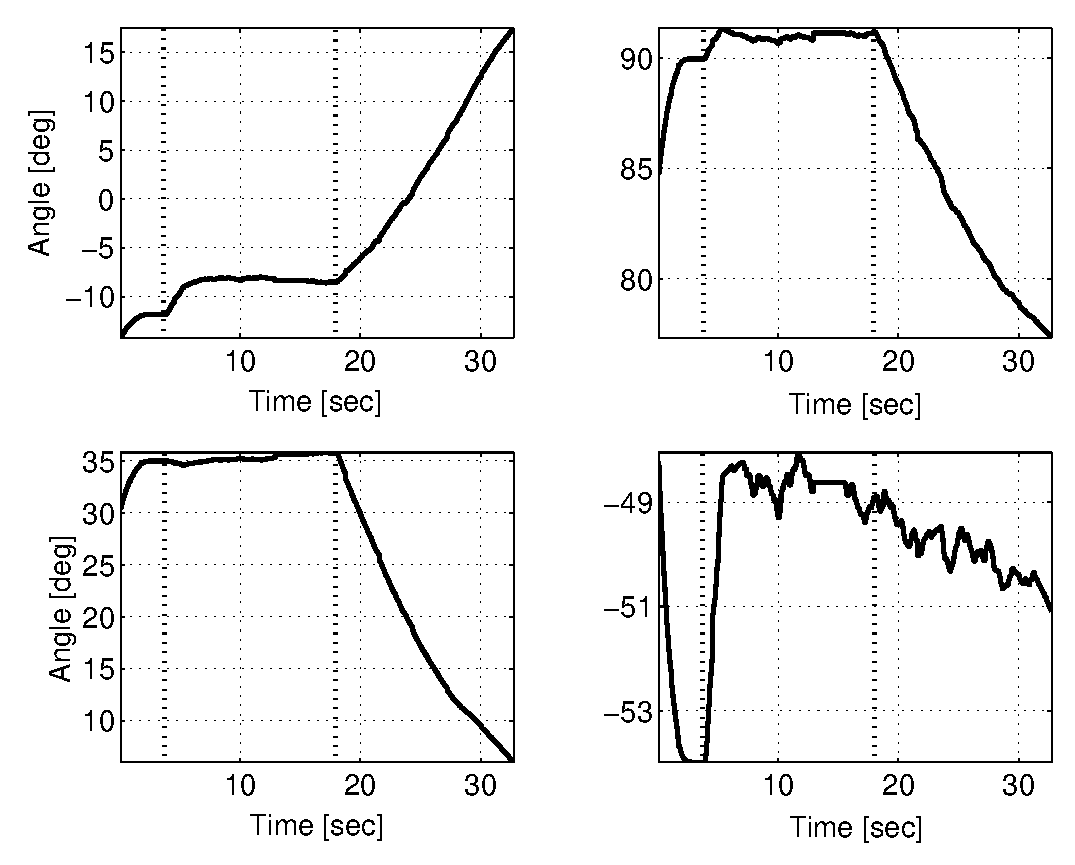
\includegraphics[width=60mm]{Figure/RedundancyArm.eps}
	\end{center}
\caption{Arm movement corresponding to the image plane movements shown in Figure \ref{Fig:RedundancyImagePlane}.
 Remarkably, the null space movement is characterized by large joint movements which are however not visible 
in the image plane due to the jacobian based compensation.} \label{Fig:RedundancyArm}
  \end{figure}